
\chapter{实验结果}
\label{cha:experiment}

在本章中,本文完整地展示了 F2000 模式分量的代码生成、编译、运行、数据分析等步骤。

\section{配置文件}

以下是用户输入的配置文件的主要部分,分别对应 models.xml , setup.xml , option.xml , field.xml ,  fakeModel.xml 五个配置文件。由于篇幅所限部分域用省略号 ... 代替,其余配置文件请参见 github 代码库 \footnote{https://github.com/NeoGeon/BCGen} 。

models.xml 下的每个model字段描述一个模式分量实现,其中主要包含模式分量名name,模式分量实现名version,数据结构attrVect,域规格domain,对外函数接口method等。以cam模式分量实现为例,该模式分量实现属于atm模式分量,因此name字段设为atm,version字段设为cam。其详细配置位于同目录下的camDesc.xml文件中,这里将metaFile字段设定为camDesc.xml以引用目标文件。其相关输入输出数据结构分为flds\_atm2x\_states,flds\_atm2x\_fluxes,flds\_x2atm\_states,flds\_x2atm\_fluxes四部分,在attrVect字段中的field字段进行注册,其具体内容在fields.xml中注册并引用。两个域规格flds\_dom\_coord和flds\_dom\_other数据结构在domain字段中进行注册,其具体内容在fields.xml中注册并引用。主要方法atm\_init\_mct,atm\_run\_mct,atm\_final\_mct在method中注册,其输入输出参数atm2x\_atmatm和x2atm\_atmatm分别在in\_args和out\_args的arg字段注册。

\begin{figure}[H]
\centering
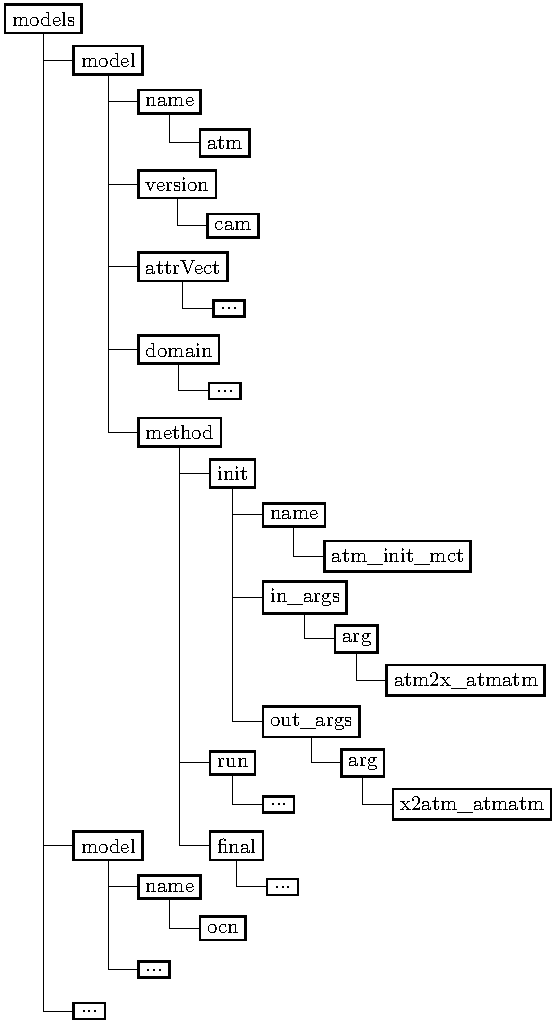
\includegraphics{../figures/models.pdf}
\caption{models.xml 结构示意图}
\end{figure}

setup.xml 下的models包含实验实例全部需要用到的模式分量实现。每个model通过name和version字段对 models.xml进行引用,其余字段为该模式分量实现在当前实验实例中使用所需的配置。特别的,input字段描述了该模式分量实现各个接口的连接方式。以cam模式分量实现为例,该模式分量通过name字段atm和version字段cam对models.xml进行引用,其分辨率为fv4x5,在res字段设置。根据相关物理模型,frac字段设为normal。cam模型输入的各个数据根据来源在input进行注册,与之相连的ocn, lnd, ice模型和xao伪模型分别在src字段的设置中记录,其field字段根据不同数据类型对各个要传输的数据分别记录,如来自ocn的So\_t数据类型为state,比率类型normal,因此在src name='ocn' 中添加field type='state' frac='normal'的字段So\_t。多个字段的情况如来自lnd模型的Sl\_fv和Sl\_ram1在src name='lnd'字段中添加field type='
state' frac='normal'的字段Sl\_fv:Sl\_ram1。

\begin{figure}[H]
\begin{minipage}[t]{0.5\linewidth}
\centering
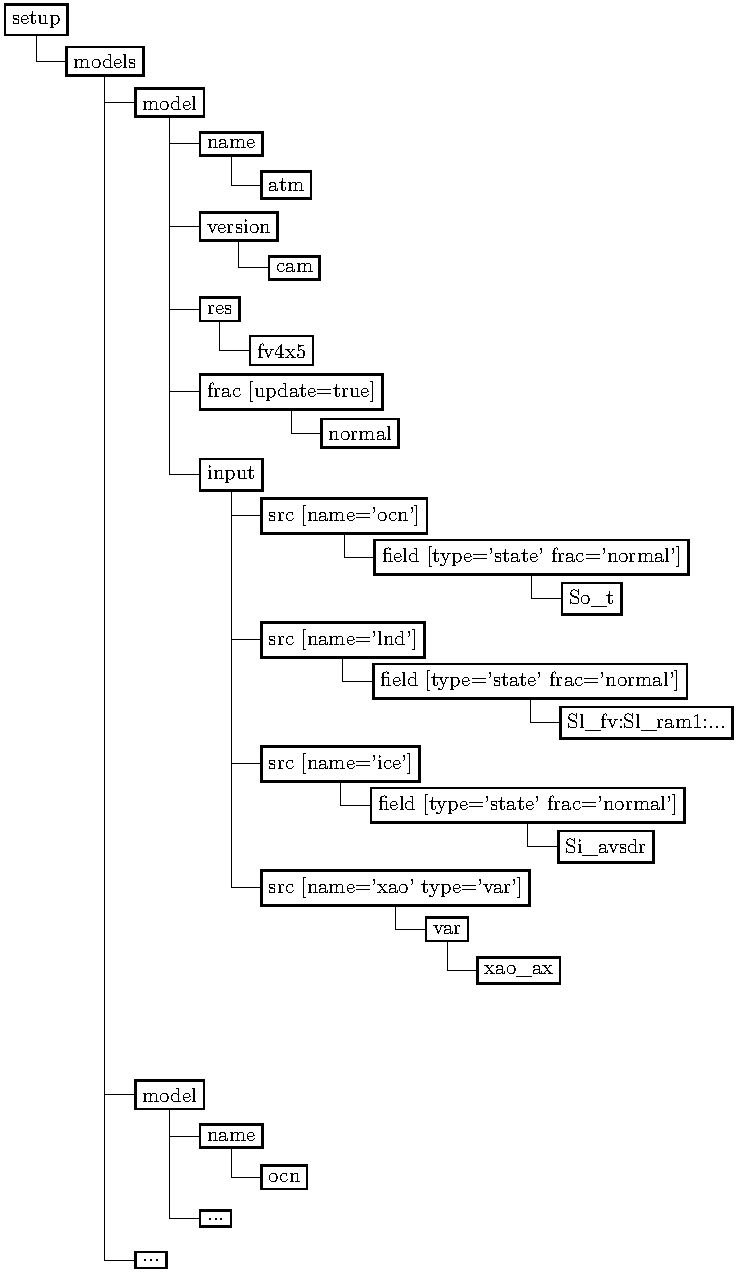
\includegraphics[height=.5\textheight]{../figures/setup.pdf}
\caption{setup.xml 结构示意图}
\end{minipage}
\begin{minipage}[t]{0.5\linewidth}
\centering
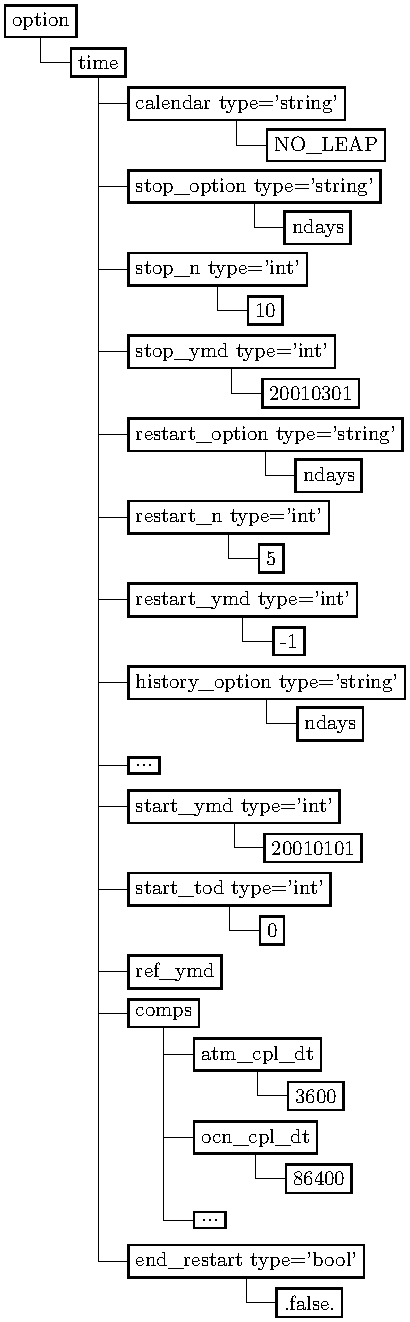
\includegraphics[height=.5\textheight]{../figures/option.pdf}
\caption{option.xml 结构示意图}
\end{minipage}
\end{figure}

option.xml 下包括各个内部库的参数设置,这里主要是time时钟模块,日期无跳跃在calendar type='string' 字段中记录NO\_LEAP,起始日期在start\_ymd type='int'字段中记录20010101,起始时间在start\_tod type='int'中记录0,停止时间在stop\_option type='string'字段中设置ndays并在stop\_n type='int'字段中设置10。重启周期在restart\_option type='string'字段中设置ndays并在restart\_n type='int'字段中设置5。历史记录周期在history\_option type='string'字段中设置ndays并在history\_n type='int'字段中设置1。各个模式分量的运行时间周期在comps字段中对各个模式分量进行记录,atm模式分量在atm\_cpl\_dt字段中记录3600,ocn模式分量在ocn\_cpl\_dt字段中记录86400。

fields.xml 对各个数据和数据结构进行了统一注册。每个数据在fldMeta字段中进行注册,包括shortname, longname, stdname, units四个字段,缺失记unknown。每个数据结构在fields字段中记录其包含的所有数据。同一数据可能被多个不同数据结构包含。flds\_dom\_coord数据结构在fields中记录为fieldVar name='flds\_dom\_coord'字段并在其中的field字段记录lat:lon,这两个数据分别在fldMeta字段中记录为fld字段,他们的shortname字段分别为lat和lon,longname字段均为unknown,stdname字段分别为latitude和longitude,units字段分别为degrees north和degrees east。

\begin{figure}[h]
\begin{minipage}[t]{0.5\linewidth}
\centering
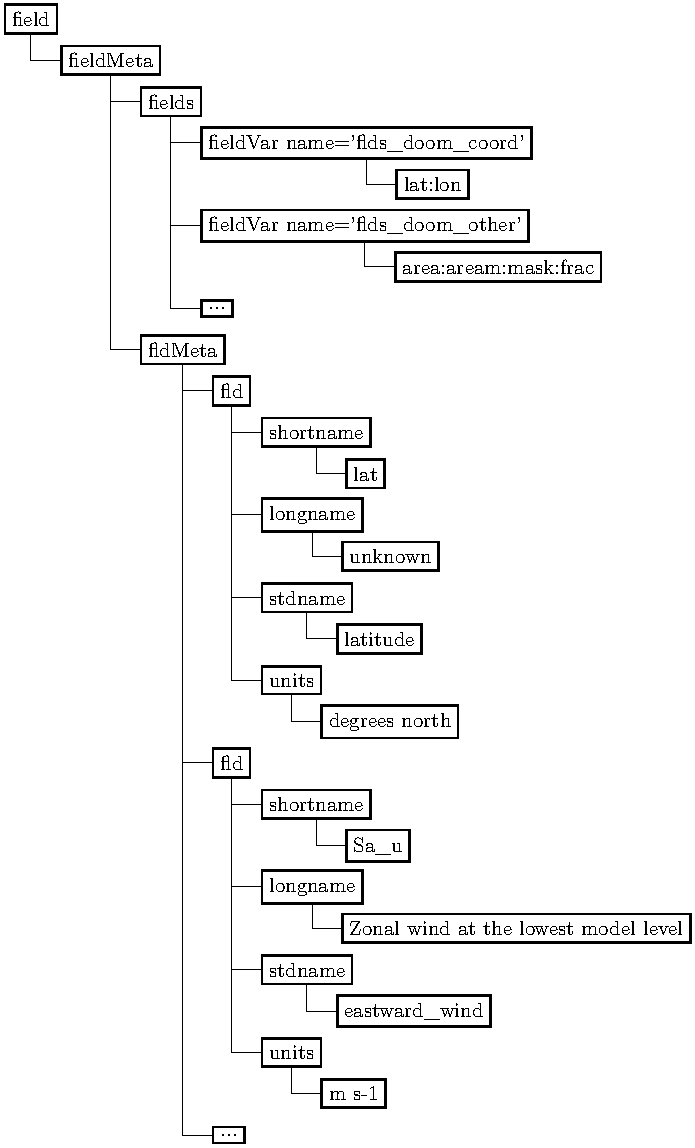
\includegraphics[height=.5\textheight]{../figures/fields.pdf}
\caption{fields.xml 结构示意图}
\end{minipage}
\begin{minipage}[t]{0.5\linewidth}
\centering
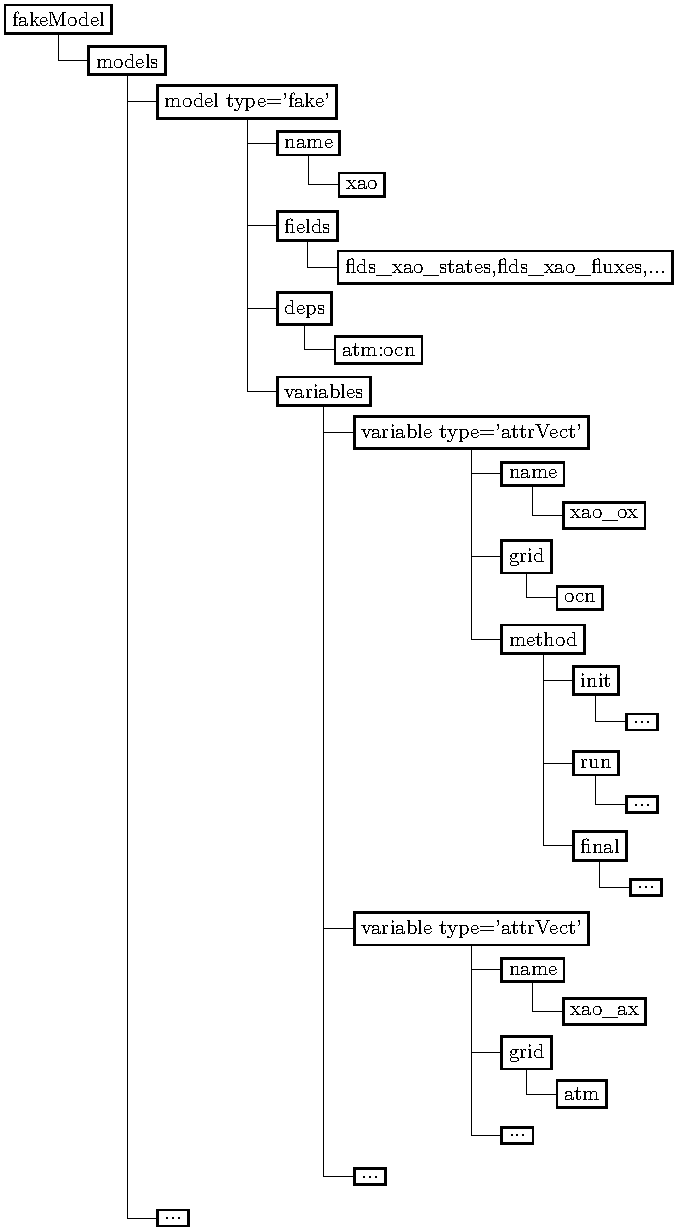
\includegraphics[height=.5\textheight]{../figures/fakeModel.pdf}
\caption{fakeModel.xml 结构示意图}
\end{minipage}
\end{figure}

fakeModel.xml 主要描述了各个特殊数据结构组成的伪模型,这里以海气通量xao为代表,其相关数据结构分为flds\_xao\_states,flds\_xao\_fluxes,flds\_xao\_fields三部分,在attrVect字段中的field字段进行注册,其具体内容在fields.xml中注册并引用。其依赖模式分量atm和ocn在deps字段中记录为atm:ocn,相关变量xao\_ox和xao\_ax分别在variables字段中记录为variable字段,以xao\_ox为例,其name字段记为xao\_ox,grid字段记录为ocn,method字段中对init, run, final三套函数在phase字段中进行注册,init阶段第一个函数name字段为flux\_init\_mct,args字段中注册的四个参数分别为gsmap, domain, mpicom, fraction,均通过ocn模型,因此在arg model='ocn'字段中分别记录。 init阶段第二个函数name字段为flux\_ocnalb\_mct,其参数有两个来源于ocn,在arg model='ocn'字段中分别记录为comp和fraction,另一个参数是该变量自身,直接在arg字段中记录xao\_ox。run和final类似。在xao\_ox和xao\_ax全部注册完毕后该文件的variables字段完成。

\section {代码生成}

在用户配置全部录入后,可以通过代码生成模块中的 instCreator 模块进行解析和代码生成。该模块会将解析出的结果以 log 的形式输出到屏幕。若配置正确,应当会产生如下输出:

\begin{lstlisting}
('name', 'atm2x_atmx')
('model', 'atm')
('fraclist', 'afrac:ofrac:lfrac:ifrac')
('init', 'fraction_atm_init')
('update', 'fraction_atm_update')
{'fraclist': 'afrac:ofrac:lfrac:ifrac', 
'init': 'fraction_atm_init', 'update': 
'fraction_atm_update', 'fracs': [{'mapper': 
'mapper_Smatocn2atm', 'model': 'ocn', 'name': 
'ofrac'}, {'mapper': 'mapper_Smatlnd2atm',
'model': 'lnd', 'name': 'lfrac'}, {'mapper':
'mapper_Smatice2atm', 'model': 'ice',
'name': 'ifrac'}]}
...
('name', 'mapper_comp_map')
('arg', 'ocn2x_ocnx')
('arg', 'ocn2x_atmx')
('attrVect', 'lnd2x_lndx')
('field', 'Sl_fv:Sl_ram1:Sl_snowh:Fall_flxdst1:
Fall_flxdst2:Fall_flxdst3:Fall_flxdst4')
...
\end{lstlisting}

\section {内部库预编译}

全部代码生成后会调用 make 工具进行自动内部库编译,若内部库和生成代码格式正确且接口符合,应当会产生如下输出

\begin{lstlisting}
make[1]: Entering directory `/home/hq/git
/protected/BCGen/baseCpl/src/logUtils'
mpif90 -c -I/home/hq/git/protected/BCGen/
baseCpl/include -L/home/hq/git/protected/
BCGen/baseCpl/lib logUtil.F90 
mv *.o /home/hq/git/protected/BCGen/baseCpl/lib
mv *.mod /home/hq/git/protected/BCGen/baseCpl/include
make[1]: Leaving directory 
...
Checking whether input datasets exist locally...
OK -- found depvel_file = /mnt/CESM-data/inputdata/
atm/cam/chem/trop_mozart/dvel/depvel_monthly.nc
OK -- found tracer_cnst_filelist = /mnt/CESM-data/
inputdata/atm/cam/chem/trop_mozart_aero/oxid/
oxid_1.9x2.5_L26_clim_list.c090805.txt
...
\end{lstlisting}

\section {生成实例}

编译后的内部库会与各个模式分量实现的代码一同创建为实验实例,其结构如下图。该实例可以直接编译运行,或对模式分量实现进行嵌入式调试。

\usetikzlibrary{trees}
\tikzstyle{every node}=[draw=black,thick,anchor=west]
\tikzstyle{selected}=[draw=red,fill=red!30]
\tikzstyle{optional}=[dashed,fill=gray!50]

\begin{figure}[H]
\begin{tikzpicture}[%
  grow via three points={one child at (0.5,-0.7) and
  two children at (0.5,-0.7) and (0.5,-1.4)},
  edge from parent path={(\tikzparentnode.south) |- (\tikzchildnode.west)}]

  \node{BCGen}
    child { node{BCGen\_inst}
    	child { node {include} 
    		child { node {这里存放内部库和各个模式分量实现的.mod文件} }
    	}
    	child [missing] {}
    	child { node {lib}
    		child { node {这里存放内部库和各个模式分量实现的.o和.a文件} }
    	}
    	child [missing] {}
    	child { node {scripts}
    		child { node {instBuild.sh 自动编译脚本} }
    		child { node {pullDeps.py 自动更新依赖脚本} }
    	}
    	child [missing] {}
    	child [missing] {}
    	child { node {src}
    		child { node {mapper.rc 部分数值文件列表}}
    	}
    	child [missing] {}
    	child { node {models}
    		child { node {cpl}
    			child { node {耦合器主代码,可自动编译为可执行文件} }
    		}
    		child [missing] {}
    		child { node {atm}
    			child { node {大气模式分量实现} }
    		}
    		child [missing] {}
    		child { node {ocn}
    			child { node {海洋模式分量实现} }
    		}
    		child [missing] {}
    		child { node {...} }
    	}
    };
\end{tikzpicture}
\caption{生成实例结构示意图}
\end{figure}

\section {数据分析}

通过 ncl\footnote{http://www.ncl.ucar.edu/Applications/maponly.shtml} 语言对输出的 NetCDF 数据进行作图,可以得出可视化结果。以下为其中一例数据结构:

\begin{figure}[H]
\centering
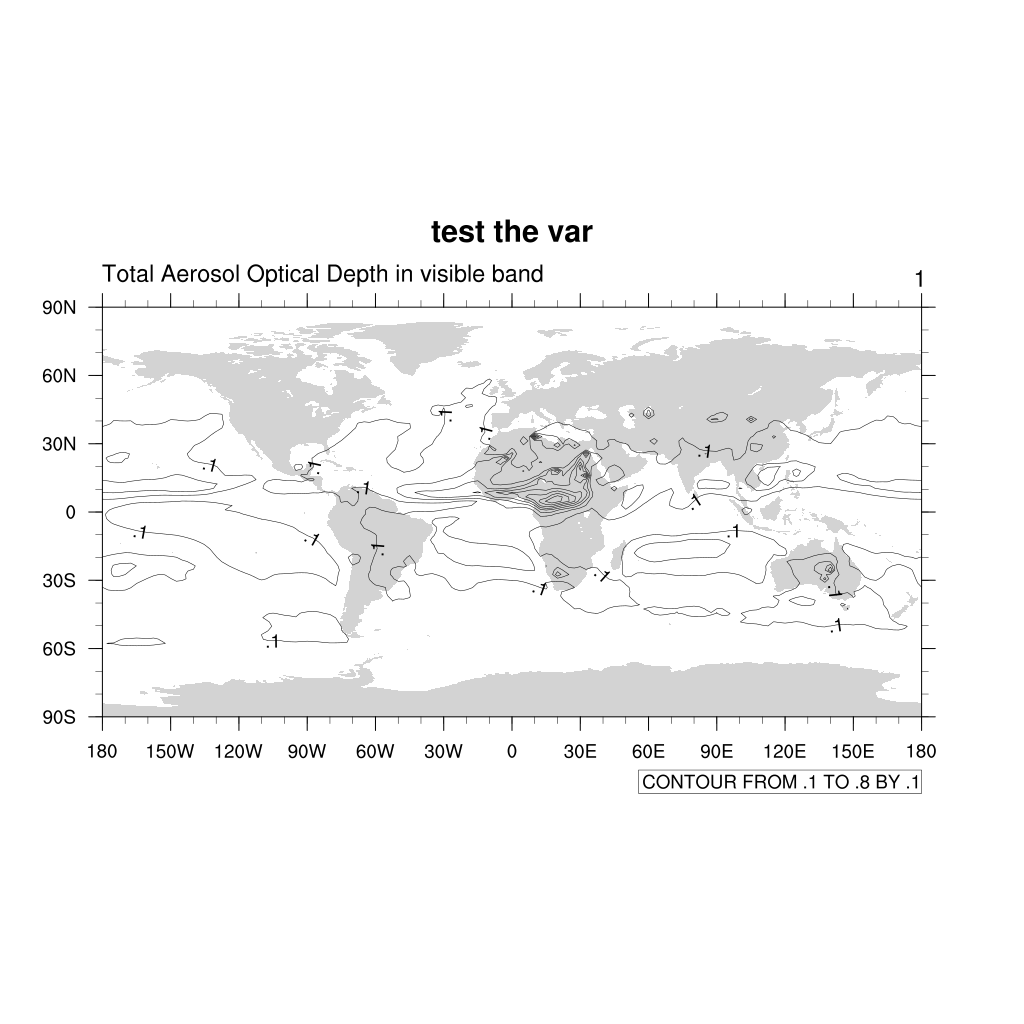
\includegraphics[width=1\textwidth]{../figures/test.png}
\caption{数据分析结果图}
\end{figure}
